\section{Theory: When Does Instance Normalization Hurt?}\label{sec:theory}

This section characterizes, in closed form, when instance normalization helps and when it hurts multi-step forecasting. We compare three level-handling strategies inside a single linear--Gaussian instance model: \rawm{} (global z-score only), \inm{} (instance normalization of the RevIN family, \citealp{kim2022revin}), and \cnm{} (conditional normalization, which estimates the target-time level from exogenous covariates), in both an oracle and an estimated variant. The analysis yields a crossover threshold $\lamstar$ in the level-predictability coordinate $\lambda$ (\Cref{eq:lamstar}), a horizon monotonicity result (\Cref{eq:prop3}), and a representational-deficiency result for affine restoration (\Cref{eq:prop1}). All formal proofs are deferred to \Cref{app:proofs}.

\subsection{Generative model and level predictability}

We posit that the observed series is driven by exogenous covariates through its level and scale,
\begin{equation}\label{eq:model}
  y_t \;=\; m(x_t) \;+\; \sigma(x_t)\, z_t ,
\end{equation}
where $x_t \in \mathbb{R}^d$ collects exogenous covariates (numerical weather predictions, installed capacity, temperature, calendar variables), $m(\cdot)$ is the covariate-determined \emph{level} function, $\sigma(\cdot)$ a conditional scale, and $z_t$ a quasi-stationary \emph{shape} component (periodicities plus weak autoregressive structure). The exogenous predictability of the level is measured by the population $R^2$ of the window mean given covariates,
\begin{equation}\label{eq:lambda}
  \lambda \;\equiv\; R^2_{\mathrm{level}}
  \;=\; 1 - \frac{\mathbb{E}\!\left[\var\!\left(\bar y_w \mid x\right)\right]}{\var\!\left(\bar y_w\right)},
  \qquad \bar y_w = \text{lookback-window mean of } y .
\end{equation}
The diagnostic of \Cref{sec:lps} is precisely a pre-training, out-of-sample estimate of \Cref{eq:lambda}.

\subsection{A stylized instance-level model (M1)}

A forecasting instance is a lookback window of $w$ steps together with a target $h$ steps ahead. Because the predictable part of the shape component is handled identically by all three strategies, we compare \emph{level-restoration} error only and absorb shape prediction into a common residual $\sigma_\varepsilon^2$ (Assumption~A3 below). Each instance draws the following independent Gaussian variables:

\begin{center}
\begin{tabular}{@{}llp{7.6cm}@{}}
\toprule
Symbol & Distribution & Role \\
\midrule
$g_T$ & $\mathcal{N}(0,\lambda V)$ & covariate-explained target-time level (\cnm{} observes it through $x$) \\
$v_T$ & $\mathcal{N}(0,(1-\lambda)V)$ & unexplained target-time level \\
$\Delta$ & $\mathcal{N}(0,\sdel)$ & covariate-\emph{orthogonal} train$\to$test shift (shared by window and target) \\
$\delta_x$ & $\mathcal{N}(0,\sx)$ & within-horizon covariate-driven level change (ramp); $g_w = g_T - \delta_x$ \\
$\delta_u$ & $\mathcal{N}(0,h\sigma_u^2)$ & within-horizon unexplained drift (random walk); $v_w = v_T - \delta_u$ \\
$\bar\varepsilon$ & $\mathcal{N}(0,\sigma_z^2/w)$ & window-mean shape noise \\
$e$ & $\mathcal{N}(0,\sest)$ & \cnm{} first-stage error, $\hat m = g_T + e$ \\
$\zeta$ & $\mathcal{N}(0,\sigma_\varepsilon^2)$ & common shape residual \\
\bottomrule
\end{tabular}
\end{center}

\noindent The derived quantities are the target-time level $L = \Delta + g_T + v_T$, the window level $M = \Delta + g_w + v_w$, the observed window mean $\bar y = M + \bar\varepsilon$, and the target $y = L + \zeta$. Here $V = \var(g_T + v_T)$ is the total level variance, so $\lambda = \var(g_T)/V$ coincides with $R^2_{\mathrm{level}}$ in \Cref{eq:lambda}. The within-horizon terms have direct physical readings: $\delta_x$ is a weather ramp or heat-wave onset that the covariates announce, while $\delta_u$ is drift the covariates cannot see.

M1 rests on four explicit assumptions.
\begin{itemize}
  \item[\textbf{A1}] \emph{(Local level)} The level is approximately constant within the lookback window; window-to-target level change is collapsed into the displacement terms $\delta_x,\delta_u$.
  \item[\textbf{A2}] \emph{(Orthogonal decomposition)} $\Delta \perp x$: level shifts explained by covariates live on the $\lambda$ axis, orthogonal shifts on the drift axis. This is why the two axes of \Cref{fig:dominance} are independent.
  \item[\textbf{A3}] \emph{(Common shape residual)} Shape predictability is identical across strategies ($\sigma_\varepsilon^2$ common); second-order effects of normalization on shape learning are ignored here and checked empirically in \Cref{sec:synthetic}.
  \item[\textbf{A4}] \emph{(\rawm{} = global mean)} \rawm{} does not track the level from the window; without loss of generality the train-set global mean is zero. Trained linear predictors relax A4 --- see Proposition~2$'$ below.
\end{itemize}

\subsection{Closed-form risk of the three estimators}

Each strategy restores a level estimate $\hat y$ before adding the (common) shape forecast. The level errors and mean-squared errors are:

\begin{center}
\begin{tabular}{@{}llll@{}}
\toprule
Method & Restoration $\hat y$ & Level error $y - \hat y$ & $\mse$ (closed form) \\
\midrule
\rawm{} & $0$ & $L + \zeta$ & $V + \sdel + \sigma_\varepsilon^2$ \\
\inm{} & $\bar y$ & $\delta_x + \delta_u - \bar\varepsilon + \zeta$ & $\sx + h\sigma_u^2 + \sigma_z^2/w + \sigma_\varepsilon^2$ \\
\cnm{}-oracle & $g_T$ & $v_T + \Delta + \zeta$ & $(1-\lambda)V + \sdel + \sigma_\varepsilon^2$ \\
\cnm{}-est & $\hat m = g_T + e$ & $v_T + \Delta - e + \zeta$ & $(1-\lambda)V + \sdel + \sest + \sigma_\varepsilon^2$ \\
\bottomrule
\end{tabular}
\end{center}

The structural asymmetry in this table is the heart of the paper. \emph{The \inm{} error contains neither $V$ nor $\sdel$}: by removing and restoring the window level wholesale, instance normalization is immune to level variance and to train--test distribution shift --- exactly the motivation of \citet{kim2022revin}, which our model preserves. The price is that the window statistic is extrapolated as a constant across the horizon, so \inm{} pays the full within-horizon displacement $\sx + h\sigma_u^2$ plus the window-noise floor $\sigma_z^2/w$. Conversely, \emph{the \cnm{} error contains no within-horizon covariate ramp}: future covariates pin the target-time level directly, so \cnm{} pays instead the unexplained level variance $(1-\lambda)V$ and the covariate-orthogonal shift $\sdel$. Neither strategy dominates; which one wins is a property of the data-generating process, governed by $\lambda$, $h$, and $\sdel$.

\subsection{The crossover}

% Propositions carry the numbering of the paper's contribution plan
% (Prop. 2 = crossover, Prop. 3 = horizon, Prop. 1 = representational
% deficiency); they are presented in pedagogical order, so the shared
% amsthm counter is set explicitly before each statement.
\setcounter{proposition}{1}
\begin{proposition}[Crossover conditions]\label{prop:crossover}
Under M1 (A1--A4):
\begin{enumerate}
  \item[(i)] Instance normalization beats the global baseline,
  $\mse_{\inm} < \mse_{\rawm}$, if and only if
  \begin{equation}\label{eq:inraw}
    \underbrace{\sx + h\sigma_u^2 + \sigma_z^2/w}_{\text{horizon extrapolation + window noise}}
    \;<\;
    \underbrace{V + \sdel}_{\text{level variance \rawm{} cannot track}} .
  \end{equation}
  \item[(ii)] Estimated conditional normalization beats instance
  normalization if and only if $\lambda > \lamstar$, where
  \begin{equation}\label{eq:lamstar}
    \lamstar \;=\; 1 \;-\; \frac{\sx + h\sigma_u^2 + \sigma_z^2/w - \sdel - \sest}{V} .
  \end{equation}
  If $\lamstar < 0$, \cnm{}-est dominates \inm{} for every $\lambda \in [0,1]$; if $\lamstar > 1$, \inm{} dominates for every $\lambda$.
\end{enumerate}
\end{proposition}

The comparative statics of \Cref{eq:lamstar} are monotone and interpretable. First, $\partial \lamstar / \partial \sdel = 1/V > 0$: the larger the covariate-orthogonal drift, the larger the region in which instance normalization is the right tool. This is a \emph{quantified} version of the original distribution-shift motivation for RevIN --- our theory does not overturn it, it delimits it. Second, $\partial \lamstar / \partial \sest = 1/V > 0$: a noisier first stage shrinks the \cnm{} region, which is why the diagnostic of \Cref{sec:lps} is deliberately evaluated out of sample. Third, $\lamstar$ falls as $h$ grows, which we state separately because it answers the ``why multi-step?'' question. (When $\sx$ itself depends on $\lambda$, as under the synthetic data-generating process of \Cref{sec:synthetic}, the closed form is replaced by a numerical root of the same equation; see \Cref{app:proofs}.)

\begin{proposition}[Horizon interaction]\label{prop:horizon}
Under M1, for either \cnm{} variant,
\begin{equation}\label{eq:prop3}
  \frac{\partial}{\partial h}\left[\mse_{\inm}(h) - \mse_{\cnm}(h)\right]
  \;=\; \sigma_u^2 + \frac{\partial\, \sx}{\partial h} \;>\; 0 .
\end{equation}
Hence the \inm{}--\cnm{} gap is strictly increasing in the horizon and $\lamstar(h)$ is strictly decreasing in $h$.
\end{proposition}

Instance normalization freezes the window statistics and carries them across all $h$ future steps; every additional step accumulates covariate-driven ramp variance and unexplained drift that the frozen statistic cannot follow, while conditional normalization re-estimates the level at the target time. Multi-step forecasting is therefore not incidental to our thesis --- it is the regime where the boundary bites hardest, as \Cref{fig:horizon} confirms empirically.

\subsection{Representational deficiency of affine restoration}

The results above treat the strategies as restoration rules. A complementary question is representational: what solutions does attaching instance normalization to a model \emph{remove} from its function class? The starting point is structural and requires no distributional assumption. Reading off the normalize--restore pipeline as implemented \citep{kim2022revin}, the composed forecast is
\begin{equation}\label{eq:equivariance}
  \hat y \;=\; \bar y \;+\; s \cdot f\!\left(\frac{x - \bar y \mathbf{1}}{s},\, g\right),
\end{equation}
where $\bar y$ and $s$ are the lookback-window mean and standard deviation and $f$ is \emph{any} backbone. Its dependence on the window mean is therefore additive with unit slope: the arguments of $f$ are centred, so no term inside $f$ can see $\bar y$ at all. Two consequences follow immediately and for arbitrary $f$. Instance normalization cannot represent a forecast that responds to the window level with any slope other than one---it is committed in advance to the assumption that the level persists exactly across the horizon---and it cannot represent any interaction between the window level and the covariates. Global $z$-scoring with the same inputs is subject to neither restriction, because it passes $\bar y$ to the backbone unchanged. Following the constrained-regression view of \citet{toner2024linear}, the affine case makes both costs exact.

\setcounter{proposition}{0}
\begin{proposition}[Representational deficiency]\label{prop:deficiency}
Let $(\bar y, g)$ be centered and jointly Gaussian with correlation $\varrho$, let the target follow
$y = a\bar y + b g + \kappa\, \bar y\, g + \eta$ with independent noise $\eta$, and condition throughout on the instance scale $s$ of \Cref{eq:equivariance}. Write $\Delta\mse$ for excess risk over the Bayes predictor. Then, comparing the level handled endogenously (\inm) against a global constant scaling (\rawm) that passes $\bar y$ through unchanged:
\begin{enumerate}
  \item[(i)] \emph{(Affine backbone.)} Let $\mathcal{F} = \{c_0 + c_1 \bar y + c_2 g\}$ be the class available to \rawm{} and $\mathcal{R} = \{c_0 + \bar y + c_2 g\} \subsetneq \mathcal{F}$ the subclass reachable by \Cref{eq:equivariance}. Then
  \begin{equation}\label{eq:prop1}
    \Delta\mse_{\mathcal{F}} \;=\; \kappa^2\left[\var(\bar y)\,\var(g) + \covop(\bar y, g)^2\right],
    \qquad \covop(\bar y, g_T) = \lambda V \text{ under M1},
  \end{equation}
  and \inm{} pays, \emph{in addition},
  \begin{equation}\label{eq:prop1b}
    \Delta\mse_{\mathcal{R}} - \Delta\mse_{\mathcal{F}} \;=\; (a-1)^2\,\var(\bar y)\,\bigl(1-\varrho^2\bigr).
  \end{equation}
  \item[(ii)] \emph{(Unconstrained backbone.)} Let the backbone range over all measurable functions. Then \rawm{} attains the Bayes risk, $\Delta\mse_{\rawm} = 0$, whereas \Cref{eq:equivariance} confines \inm{} to $\{\bar y + \varphi(g)\}$ and its excess risk converges to the strictly positive floor
  \begin{equation}\label{eq:prop1c}
    \Delta\mse_{\inm} \;=\; \Bigl[(a-1)^2 \;+\; \kappa^2\var(g)\Bigr]\,\var(\bar y)\,\bigl(1-\varrho^2\bigr).
  \end{equation}
\end{enumerate}
\end{proposition}

Part~(i) is a projection argument: for centered jointly Gaussian variables the interaction $\bar y\, g$ is orthogonal to the linear directions $\bar y$ and $g$ (Gaussian third moments vanish), so its projection onto the class is the constant $\mathbb{E}[\bar y\, g] = \covop(\bar y, g)$, and Isserlis' theorem evaluates the variance of the residual (\Cref{app:proofs}). Within the affine class the interaction cost \Cref{eq:prop1} is paid by \rawm{} as well, so it explains no part of the gap between the two \emph{there}; what separates them is \Cref{eq:prop1b}, the price of pinning the window-mean coefficient to one, discounted by $(1-\varrho^2)$---the extent to which the covariate can stand in for the window mean and absorb the mismatch.

Part~(ii) is what makes the boundary a boundary rather than a small-sample artifact, and it reverses the intuition that flexibility fixes things. As the backbone class grows, \rawm's disadvantage is absorbed---an unconstrained model given $\bar y$ and $g$ can represent the interaction and reaches the Bayes risk---while \inm{} converges to a floor it can never cross, because no member of $\{\bar y + \varphi(g)\}$ is a function of $\bar y$ beyond the unit term. Consequently the \emph{gap} $\Delta\mse_{\inm} - \Delta\mse_{\rawm}$ does not shrink with capacity: it grows, from $(a-1)^2\var(\bar y)(1-\varrho^2)$ in the affine case to \Cref{eq:prop1c}, the difference being the interaction term $\kappa^2\var(g)\var(\bar y)(1-\varrho^2)$ which migrates from a shared cost to an \inm-only one. This is the theoretical counterpart of the two empirical patterns \Cref{sec:empirical} reports side by side: the \rawm-versus-\cnm{} gap narrows along the capacity ladder, while the \inm-versus-\rawm{} difference does not vanish at any capacity we ran.

Both parts are corollaries of \Cref{eq:equivariance}, which needs no distributional assumption at all: subtracting the window statistic before the backbone commits the model to a fixed, unit-slope, non-interacting use of the level, and downstream flexibility does not restore what that commitment removes---it merely stops helping the unconstrained alternative catch up.

Three hypotheses carry real weight and we flag them rather than burying them in the proof. \Cref{eq:prop1} needs joint Gaussianity: it is Isserlis' fourth-moment identity, and under a heavier-tailed elliptical law with the same first two moments the true interaction cost is larger. \Cref{eq:prop1b,eq:prop1c} do \emph{not} need Gaussianity---only vanishing third cross-moments---but they do need $g$ to be centered; with $\mathbb{E}[g] \neq 0$ the factor $(a-1)^2$ becomes $(a-1+\kappa\,\mathbb{E}[g])^2$, which matters in practice because covariates are standardized on the training segment and so are only approximately centered out of sample. And conditioning on $s$ is what makes $\mathcal{R}$ a subclass of $\mathcal{F}$: with $s$ varying across instances, \Cref{eq:equivariance} reaches directions ($s$ and $s\,g$) that $\mathcal{F}$ does not, and the two classes are non-nested.

\subsection{From restoration rules to trained predictors (Proposition~2$'$)}

M1's estimators are \emph{pure} restoration rules, but a trained linear backbone additionally regresses on its input window and thereby tracks residual level in distribution --- an implicit, partial instance normalization that strengthens the operational \rawm{} and \cnm{} arms beyond their M1 idealizations (a relaxation of A4). The restoration-rule threshold \Cref{eq:lamstar} is therefore an \emph{upper bound} on the crossover realized by trained linear models. Proposition~2$'$ (stated formally in \Cref{app:proofs}) replaces it with the exact object: for each normalization class the optimal linear predictor is a constrained least-squares problem with a closed-form solution \citep{toner2024linear}, solved on the training segment and evaluated out of sample, with no stochastic optimization involved. Under the baseline synthetic parameters the M1 threshold at $h=24$ is $\lamstar \approx 0.27$--$0.28$, whereas the constrained-least-squares theory --- and the trained RLinear models of \Cref{sec:synthetic} \citep{li2023rlinear} --- place the crossing far lower; the gap between the two thresholds is itself a measurement of how much implicit level tracking linear backbones perform, a point we return to in \Cref{sec:discussion}. All quantitative adjudication in \Cref{sec:synthetic} uses the exact constrained-least-squares theory; M1 is retained as the interpretable layer that explains \emph{why} the crossover exists.

\begin{figure}[t]
  \centering
  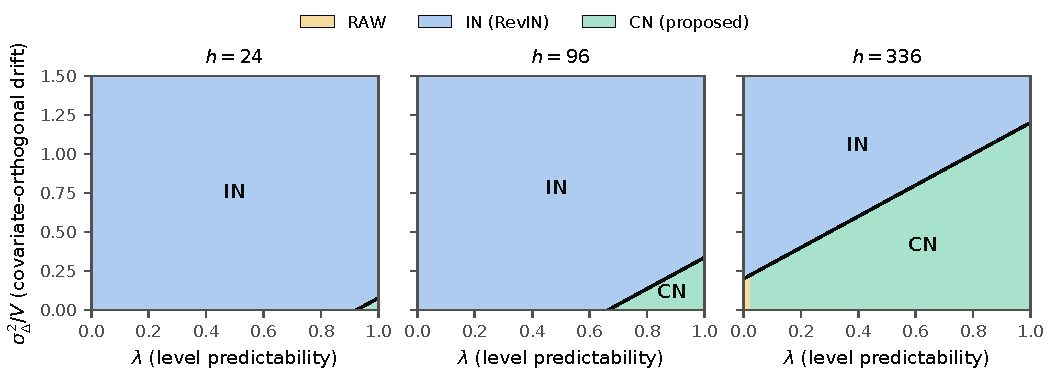
\includegraphics[width=\textwidth]{figures/fig1_dominance.pdf}
  \caption{Dominance map of the three estimators in the $(\lambda,\, \sdel/V)$ plane for $h \in \{24, 96, 336\}$ (left to right). Each region colors the argmin of the closed-form MSEs of \rawm{}, \inm{}, and \cnm{}-est under M1; the curve is the boundary $\lamstar(\sdel)$ of \Cref{eq:lamstar}. Baseline parameters: $V=1$, $w=96$, $\sigma_z=1$, $\sigma_u^2=0.0036$, $\sest=0.02$, $\sx=0$, $\sigma_\varepsilon=0$. On the drift-free axis ($\sdel=0$) the threshold is $\lamstar=0.923$ at $h=24$ and $0.664$ at $h=96$, and $\lamstar<0$ at $h=336$, where \cnm{} dominates for every $\lambda$. Takeaway: as the horizon grows, the \inm{} region retreats upward --- instance normalization survives only under large covariate-orthogonal drift, the regime its original motivation targets.}
  \label{fig:dominance}
\end{figure}

\Cref{fig:dominance} assembles the propositions into a single picture. At short horizons instance normalization is the right default across most of the plane, and covariate-orthogonal drift ($\sdel$) only enlarges its region --- the RevIN regime. As $h$ grows, the within-horizon displacement $\sx + h\sigma_u^2$ accumulates, the boundary $\lamstar(\sdel)$ sweeps down and left, and by $h=336$ conditional normalization dominates at every level of exogenous predictability unless drift is extreme. The remainder of the paper estimates the abscissa of this map from data before training (\Cref{sec:lps}), verifies the predicted boundary on synthetic data whose parameters we control (\Cref{sec:synthetic}), and tests its sign predictions on real series (\Cref{sec:empirical}).
